%=========================================================================
% fig-tuning-vectorization-pooling-access.tex
%=========================================================================

\begin{figure*}[t]

  \centering
  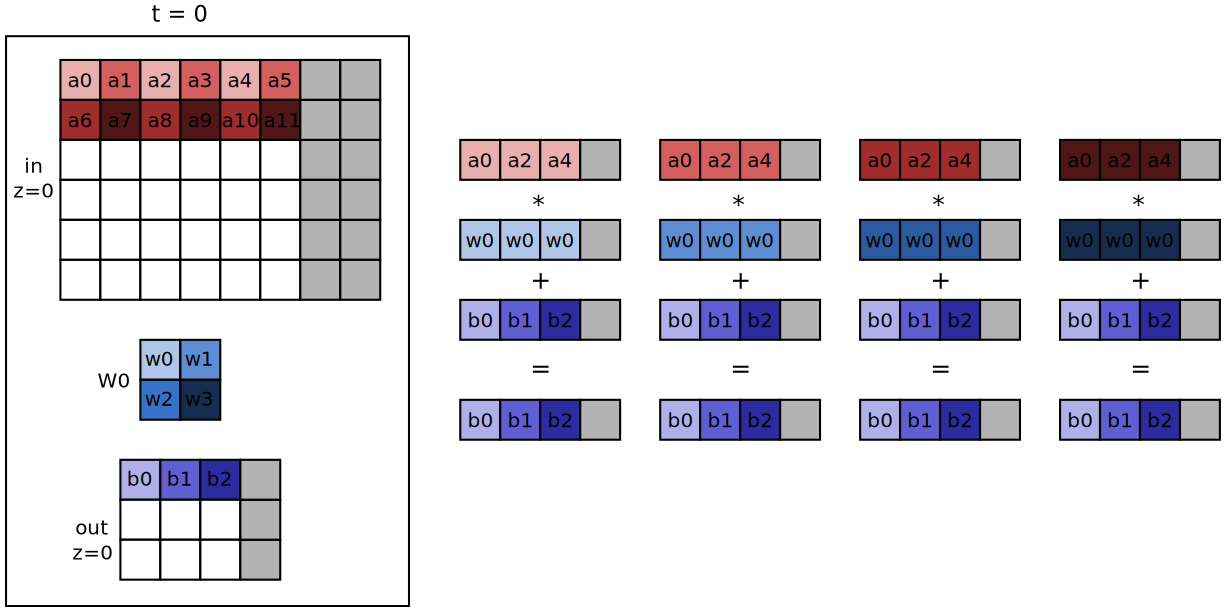
\includegraphics[width=0.9\tw]{fig-tune-vector-pooling-access.svg.pdf}

  \caption{\textbf{Memory Access Pattern for Pooling Layer --}
    Breakdown of the vector operations required to compute the first row
    of the output in a pooling layer. Each element in the vector
    corresponds to a separate element in the output. A strided load is
    used to load the input elements since the filter is applied with a
    non-unit stride for pooling layers. Otherwise, the same multiply-add
    accumulation occurs as in the convolutional layer. This example shows
    an example of padding the memory layout of the input and output so
    that vector loads/stores do not access unallocated memory.}

  \label{fig-tuning-vectorization-pooling-access}

\end{figure*}
